\chapter{An Interface For Trails} \label{chap:TrailInterface}
To facilitate the creation and exhibition of trails on a website, it is important to provide and interface that presents visual and contextual aid to the users as they are planning a path or exploring other paths. This chapter describes the two main methods used to provide such information via a Map Interface (discussed in section \ref{mappingPlatform}), and an Elevation Profile (discussed in section \ref{elevationProfile}. We discuss the decisions made and technologies used to provide these features.

\section{Mapping Platform Providers} \label{mappingPlatform}
The application provides an interactive map interface that users use to create trails. Trails are created by users clicking on points on the map. The system then calculates path between each two points created and connects to ensure that trails stay on the defined paths on the map.

To provide this, we need to use an open source map provider for the interface. In industry, there really three main providers: Google Maps, Mapbox and Ordinance Survey Maps. A comparison of these providers is shown in \autoref{tab:MappingPlatformsComparison} to help inform the decision on the chosen map provider.

To decide on what provider to use, I compare the benefits and negatives of all three in table \ref{tab:MappingPlatformsComparison}.

\begin{table}[htb!]
    \centering
    \begin{tabular}{lll}
        \hline
        \multicolumn{1}{c}{Map Provider} & \multicolumn{1}{c}{Advantages} & \multicolumn{1}{c}{Disadvantages} \\ 
        \hline
        \hline
        Google Maps & \begin{tabular}[c]{@{}l@{}}Very Accurate Map\\ Open Source Software\end{tabular} & Not very customisable \\
        \hline
        Mapbox & \begin{tabular}[c]{@{}l@{}}Open source software\\ Very customisable\\ Big community\\ Good documentation\end{tabular} & Relies on open sourced data \\
        \hline
        OS Maps & Maps are the most detailed & \begin{tabular}[c]{@{}l@{}}Not opened source\\ Only has UK map\end{tabular} \\ 
        \hline
    \end{tabular}
    \caption{Comparison of the different mapping providers that I could use}
    \label{tab:MappingPlatformsComparison}
\end{table}

Due to its big community and good documentation, Mapbox was the most suitable provider for this project. These reasons ensured development was a straightforward endeavour as there was a wealth of assistance available. Mapbox is also the map provider used by most of the example trail running applications discussed in \autoref{sec:TrailRunningApplications}, giving confidence by the fact that the provider has been tested and proven by other applications.


\subsection{Creating a Trail}
When a user clicks on the map, the system returns the coordinates of the point the user clicks on the map as shown in listing \ref{listing:exampleCoordinates}.

\begin{listing}[ht]
\caption{Example of coordinates returned from mapbox}
\inputminted[frame=lines,framesep=2mm,baselinestretch=1.2,fontsize=\footnotesize]{json}{listings/example-coordinates.json}
\label{listing:exampleCoordinates}
\end{listing}

We can use this data to draw points on the map interface, visually showing the points the user has clicked as shown in \autoref{fig:SinglePointCreated}.

\begin{figure}[ht]
    \centering
    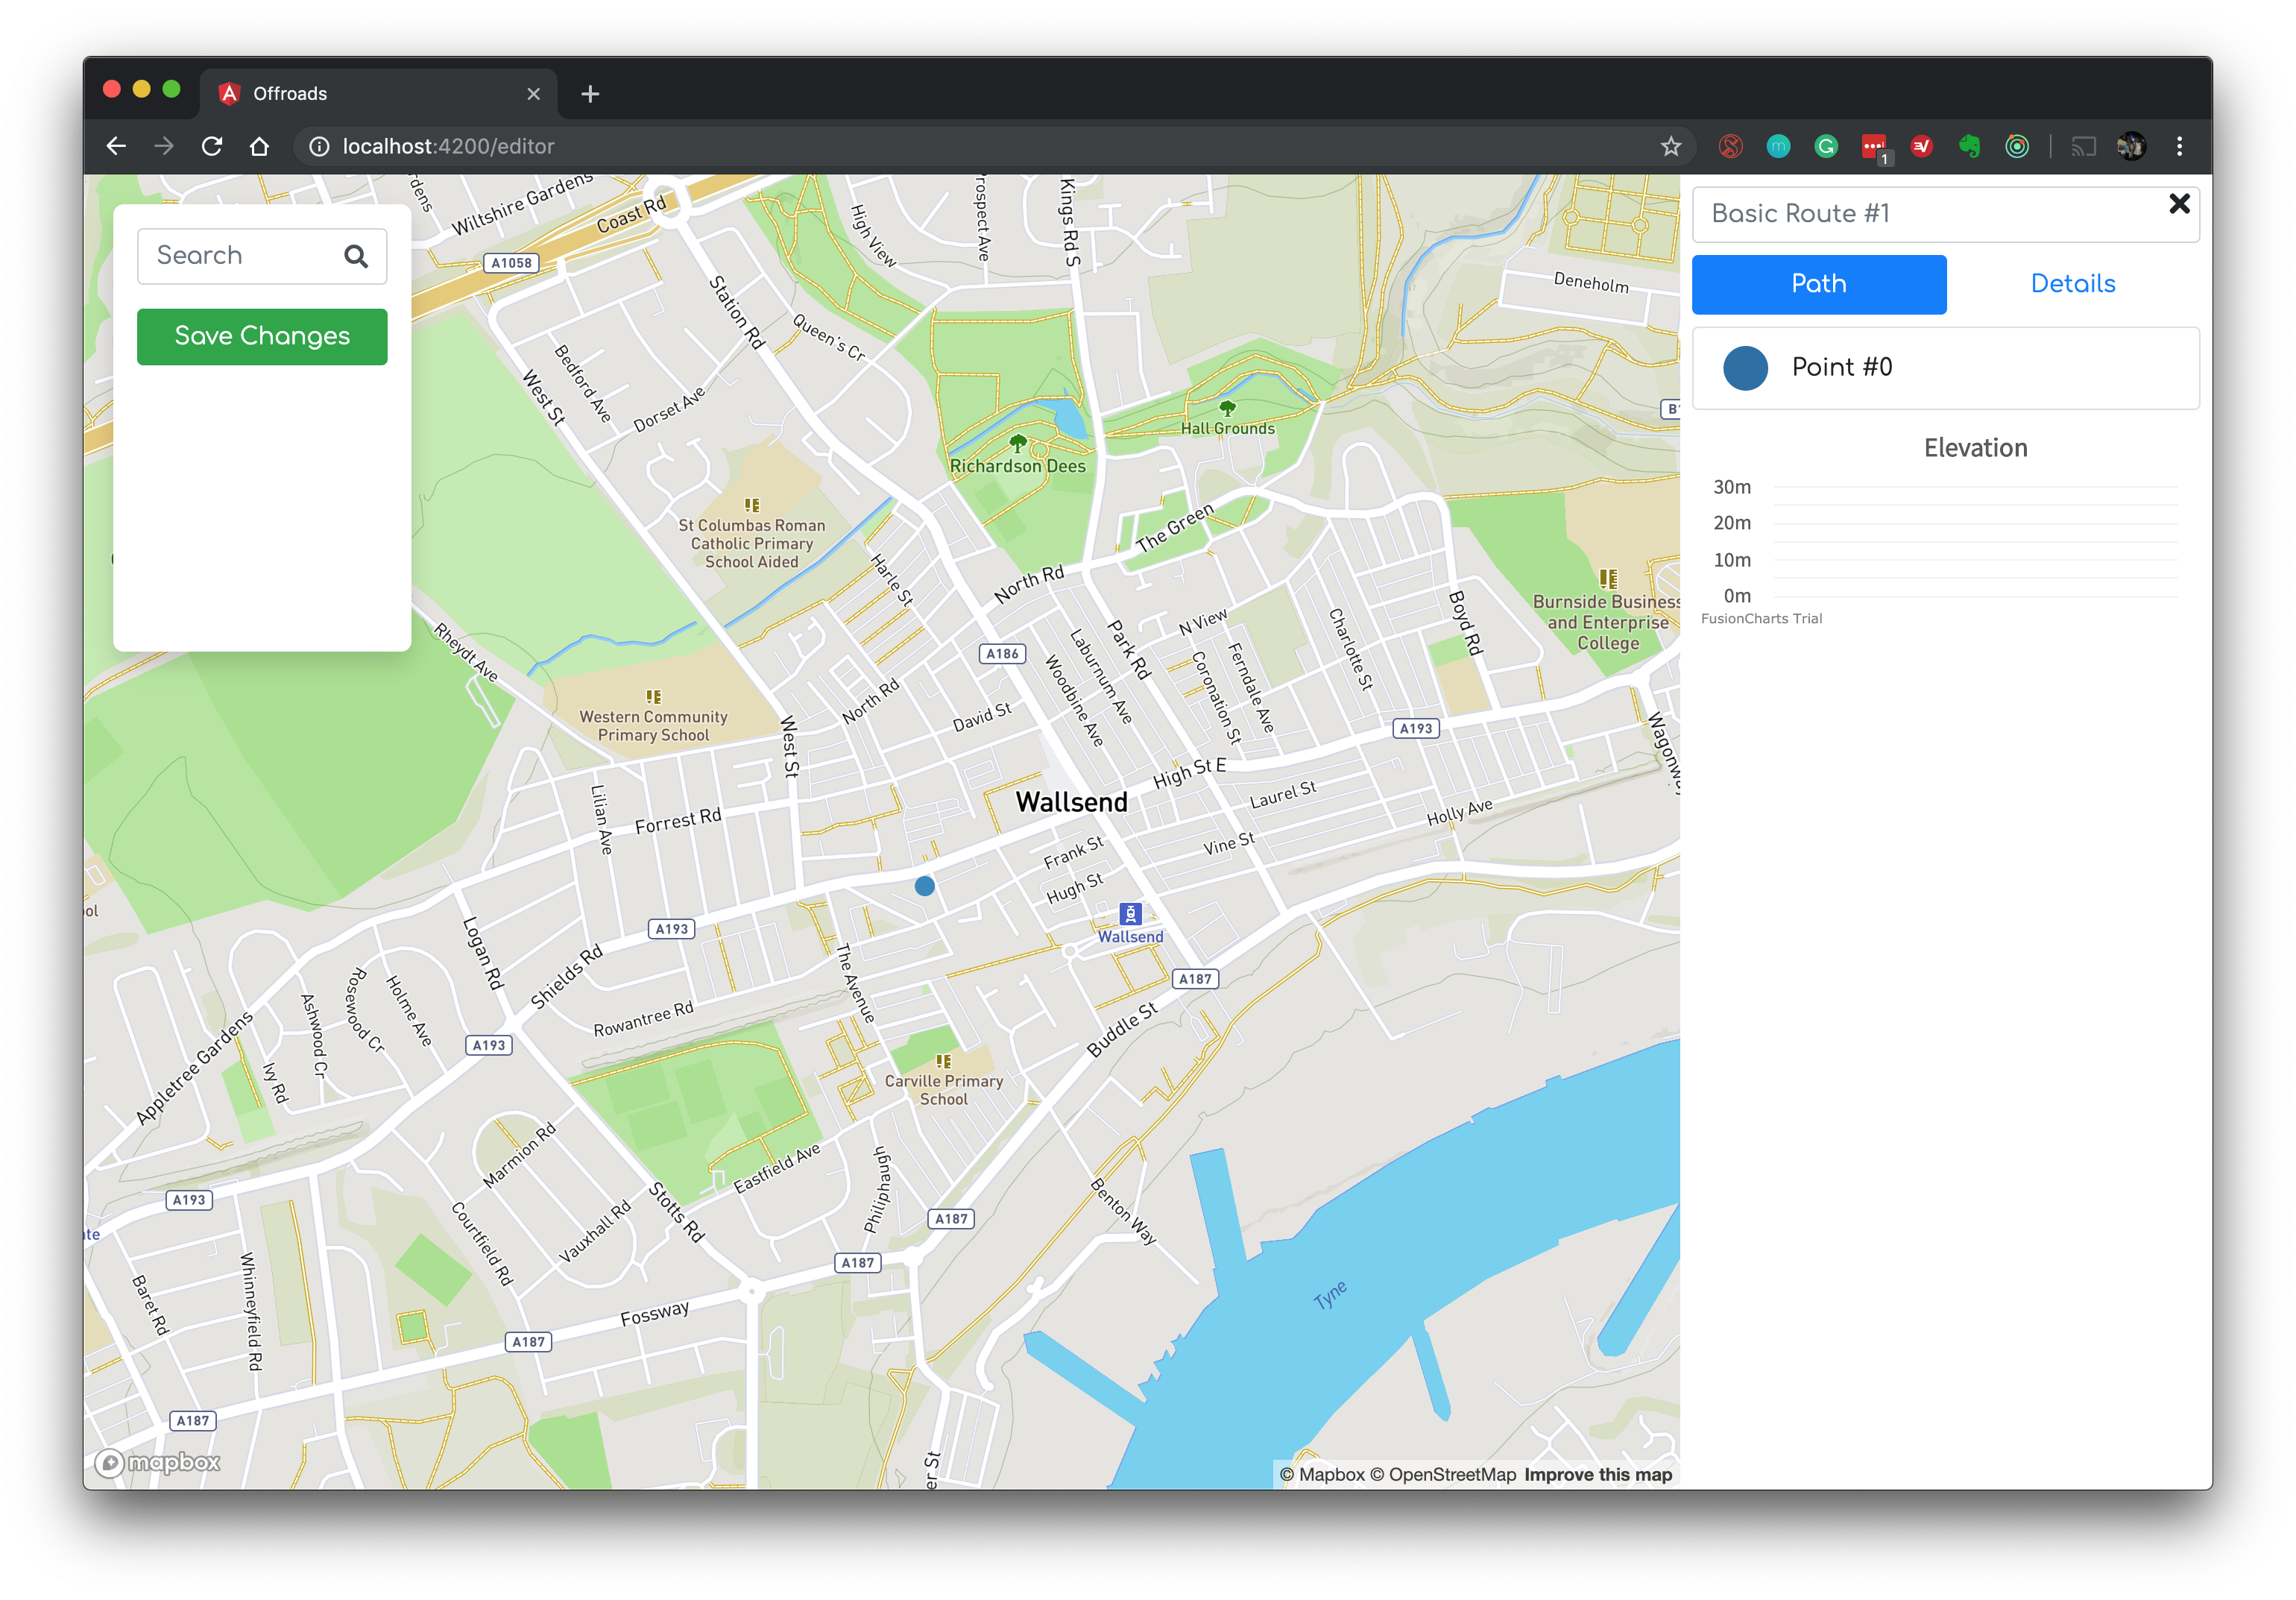
\includegraphics[width=0.75\textwidth]{single-point-on-map.png}
    \caption{The point created by a user clicking on the map indicating the location the user clicked in}
    \label{fig:SinglePointCreated}
\end{figure}
When the user adds an extra point, the system needs to combine these two points with a line. At this point, we need to calculate a path between the last point added and the new point that's just been added. When a user creates a path, it makes more sense for the path to follow already existing paths rather than a straight line that may cross over paths and terrains. Hence we need to calculate a path from between the two points to draw the line. Mapbox provides a Directions \acrshort{api} to help us do this.


\subsubsection{Finding a path}
Mapbox's Direction \acrshort{api} allows us to find a path between two points by querying the \acrshort{api} with a \textit{start} and \textit{end} coordinates.  The \acrshort{api} then returns us a a \acrshort{json} object describing the path between the specified starts and end points and the distance between the two points specified (an example is shown in appendix \ref{appSec:mapboxDirections}). We we use this data to draw a line between the two points that will follow the path returned (see figure \ref{fig:PathCreated}).

\begin{figure}[htb!]
    \centering
    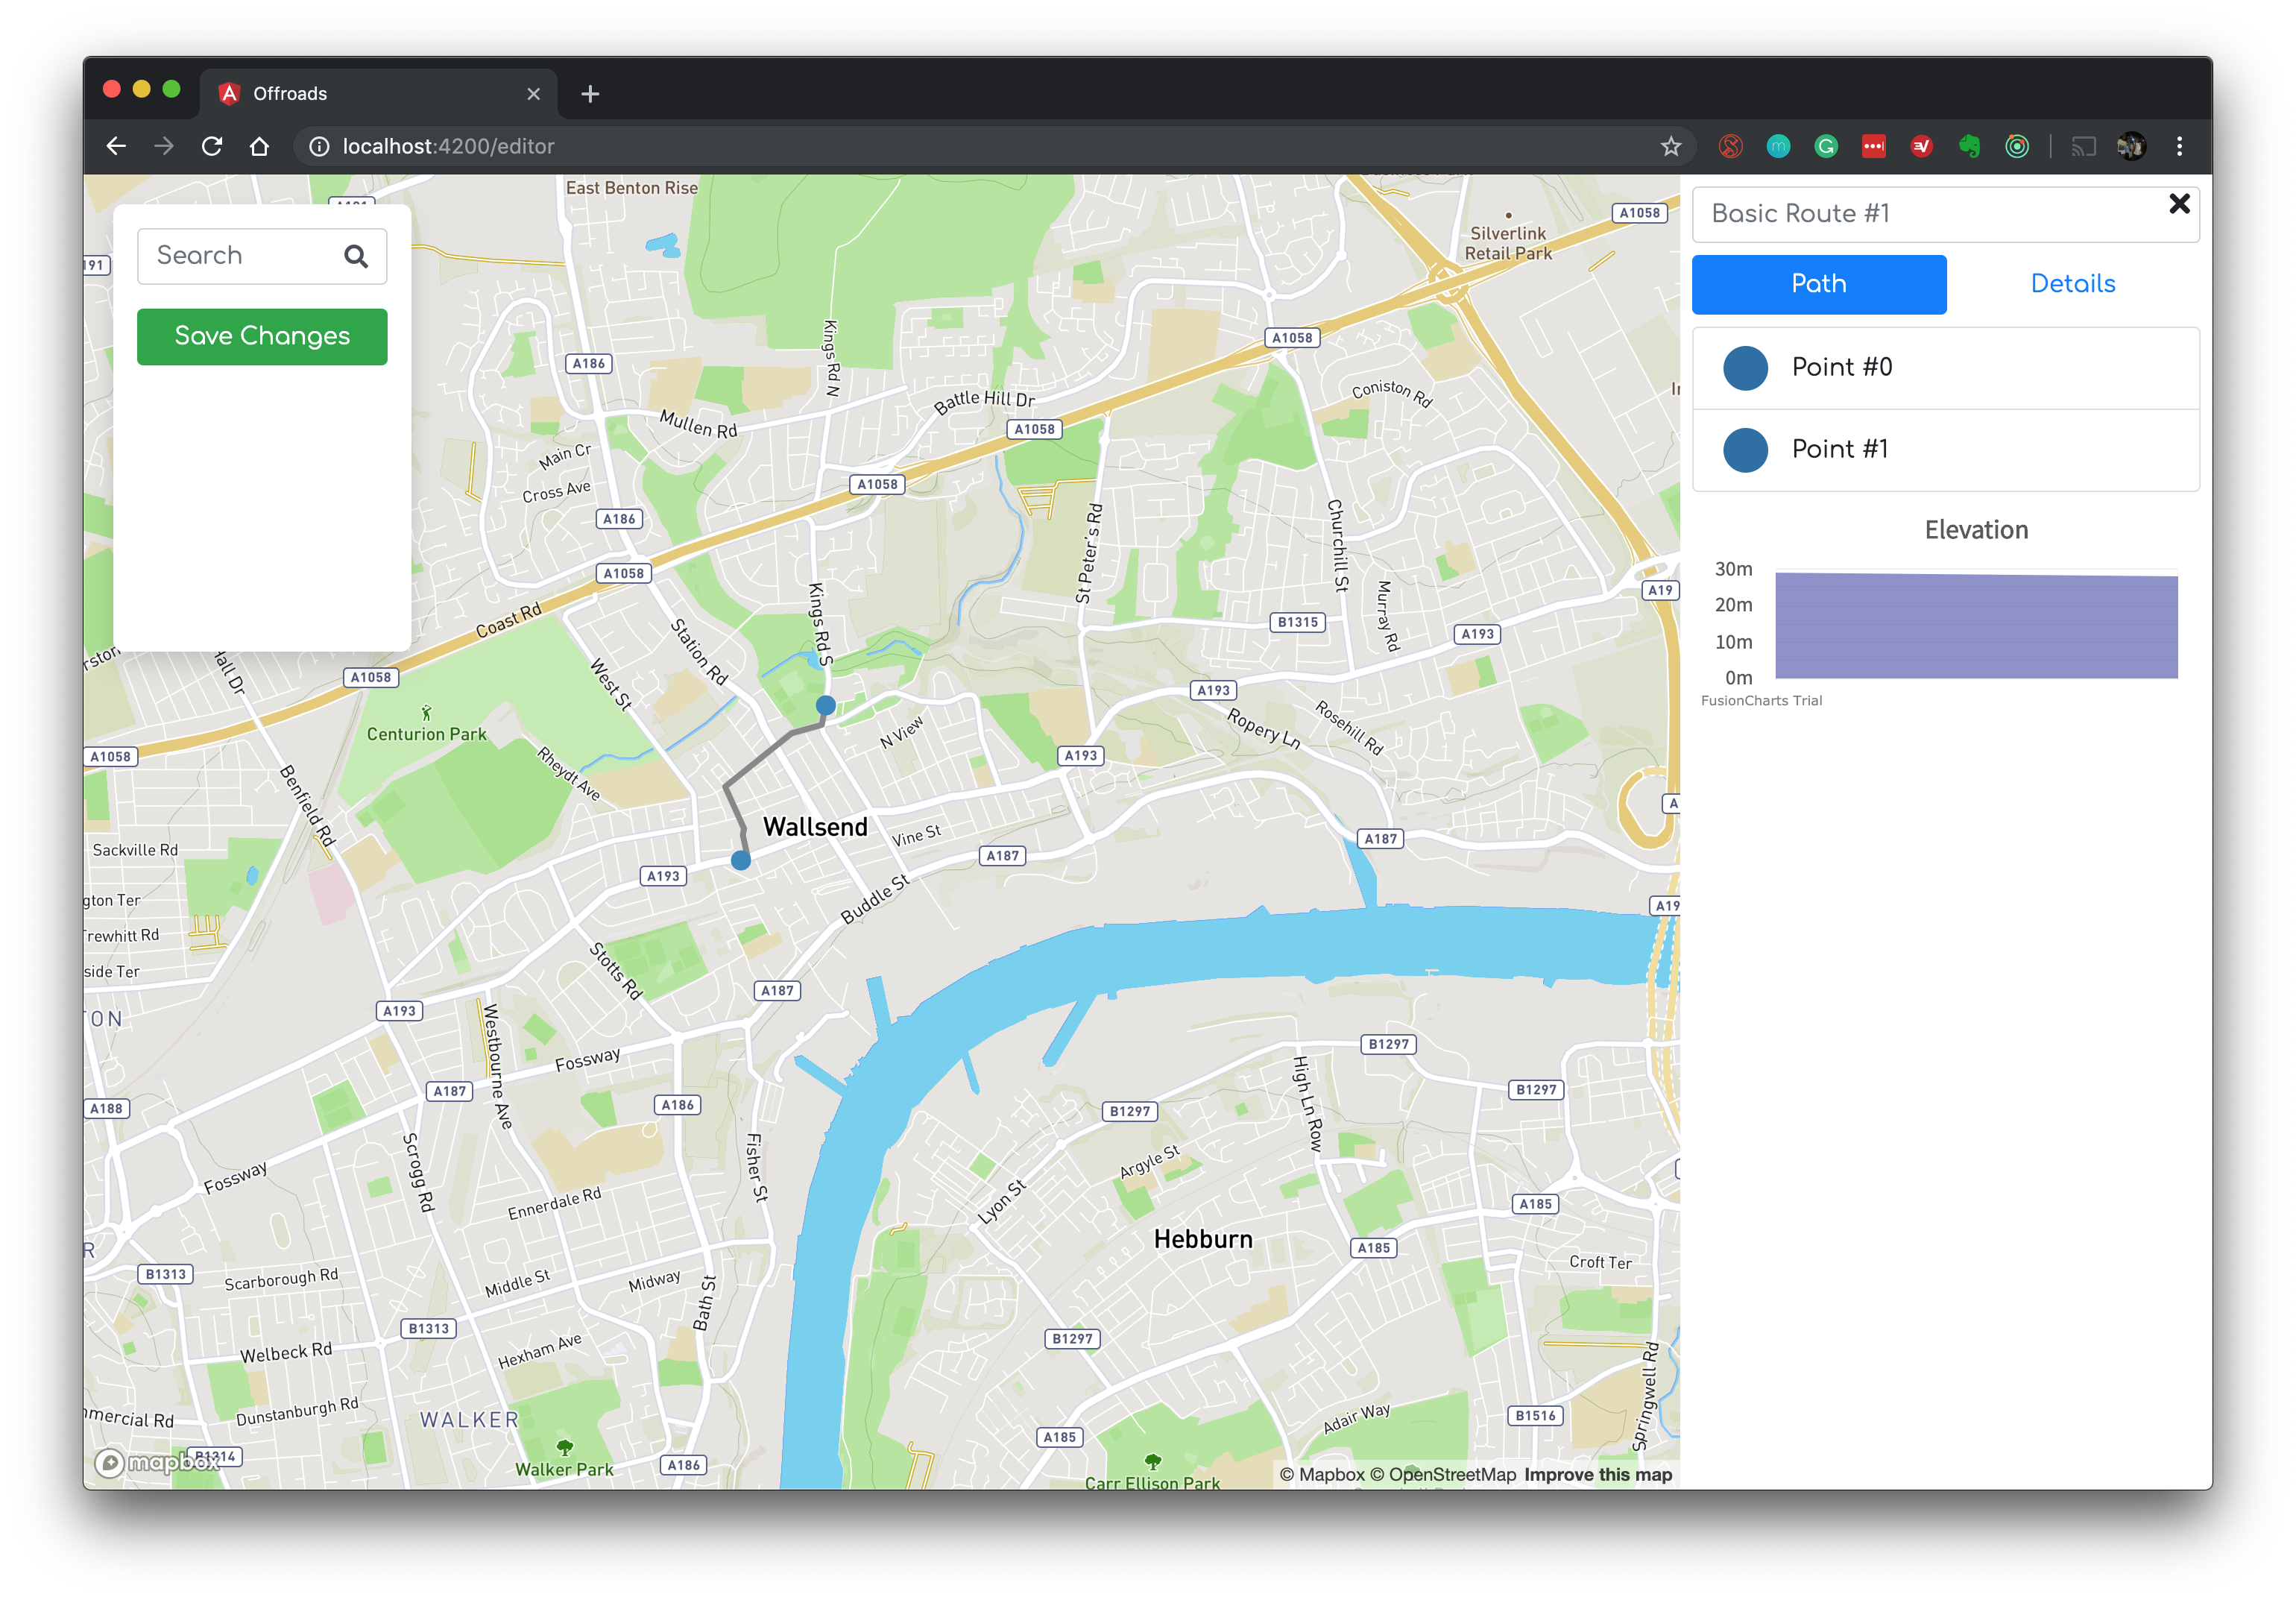
\includegraphics[width=0.75\textwidth]{path-between-points.png}
    \caption{Path created from the directions returned by the Mapbox API}
    \label{fig:PathCreated}
\end{figure}

\section{Presenting Elevation Profiles} \label{elevationProfile}
Trail runner's often use the elevation of a trail to help decide the type of trail that they wish to run. For this, the map interface provides contours that allow users to anticipate the steepness of the trail that they are creating or that they wish to run as shown in figure \ref{fig:MapContours}.

\begin{figure}[htb!]
    \centering
    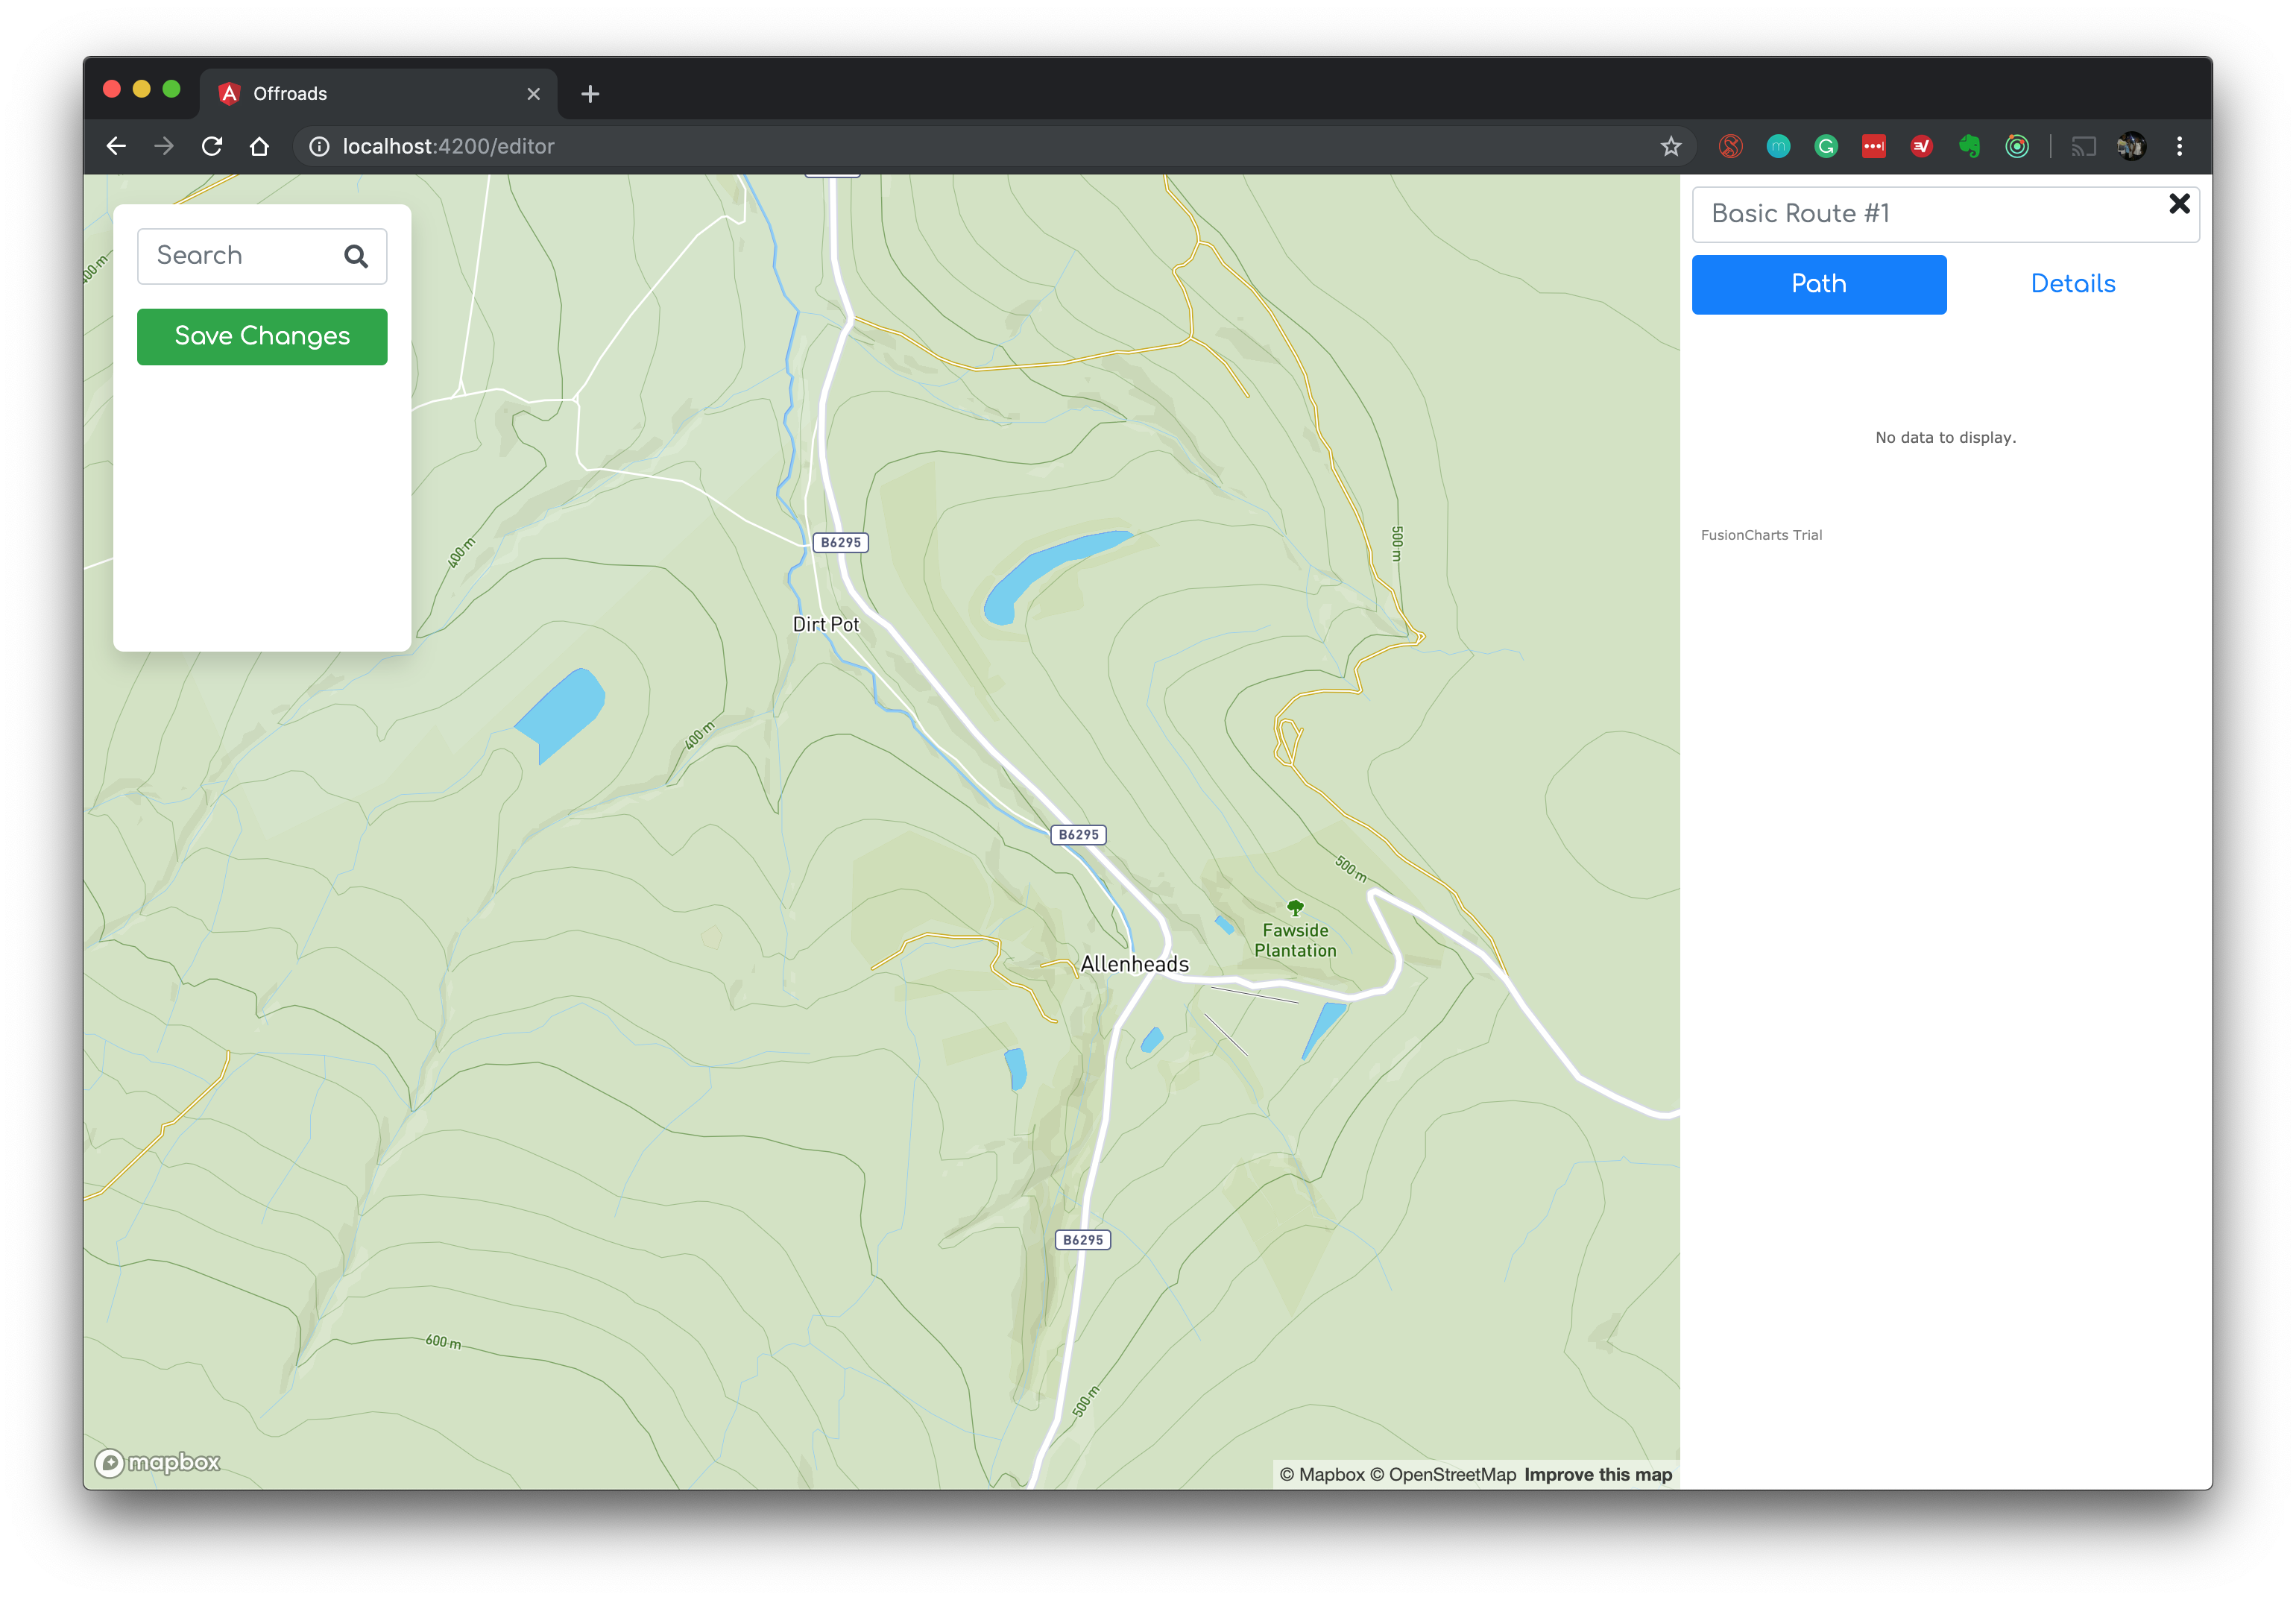
\includegraphics[width=0.75\textwidth]{map-contours.png}
    \caption{Contours on the map to help find elevation}
    \label{fig:MapContours}
\end{figure}


However, for the uninformed, reading contours can prove to be an unusual task. A better way of representing the elevation profile of is via a Graph. This will allow the user to view the elevation of a route against the distance of the route, giving a more detailed view of the elevation of the trail.

The Mapbox Directions API only provides an elevation of specific way-points of the path that is returned as shown in appendix \ref{appSec:mapboxDirections}. Although this provides some elevation information, it is not sufficient enough as the elevation of a trail can change drastically withing way-points.

Google offers an elevation service that allows you to query a trail and returns a detailed elevation profile of that trail as shown in appendix \ref{appSec:googleElevation}. As a trail is being created, we send another request to the Google elevations service to get this information. We then plot on the graph the line the line that is returned, updating it as we trail is updated. The graphing \acrshort{api} that we use is Fusion Charts \cite{fusionCharts}.